\title{Welcome to Informatica Intelligent Cloud Services}

\author{Sandeep Khandelwal}
\affiliation{%
  \institution{Indiana University}
  \city{Bloomington} 
  \state{IN} 
  \postcode{47408}
  \country{USA}
}
\email{skhande@iu.edu}

% The default list of authors is too long for headers}
\renewcommand{\shortauthors}{S. Khandelwal}

\begin{abstract}
	
In today's world data has different format (structured data,
semi-structured and unstructured data), high volume (data size is upto
hundreds of terabytes) and high velocity (amount of data getting
generated per second is too huge). Also, There is massive amount of
on-premise and cloud-based data.  Every organization has a necessity
to integrate such kind of data between on-premise and cloud-based
systems for synchronization, replication or building warehouse for
analysis and reporting purpose. Informatica Intelligent Cloud Services
(IICS)~\cite{hid-sp18-511-iics} provide complete suite of integration for such kind of diverse
and unique requirement.

\end{abstract}

\keywords{hid-sp18-511, IICS, Informatica, ETL, Data Integration}


\maketitle


\section{Introduction}

Informatica Intelligent Cloud Services is built on micro service
architecture and provide capability of data integration between
cloud-based and on-premise systems. Informatica Intelligent Clod
Services IICS~\cite{hid-sp18-511-iics} provide integration capability
in four areas mainly Integration Cloud, Data Quality and Governance
Cloud, Master Data Management Cloud, and Data Security Cloud.

\section{Integration Cloud}

Integration Cloud~\cite{hid-sp18-511-iics} product provide easy to use framework for developing data integration engine between on-premise and cloud-based systems. It has high performance data transformations to massage the data in desired format. It has push-down optimization capability to move the data processing logic to database itself instead of retrieving the data and performing the operations.It has connectivity with cloud based databases like Amazon Redshift~\cite{hid-sp18-511-aws-redshift}, Microsoft Azure SQL Data Warehouse~\cite{hid-sp18-511-ms-azure-sql}, Google BigQuery~\cite{hid-sp18-511-google-bigquery}, and Snowflake~\cite{hid-sp18-511-snowflake}.

Integration Cloud has the capability integrate the cloud based system Salesforce~\cite{hid-sp18-511-salesforce} with on-premise systems in real time using RESTfuls APIs.

\section{Data Quality and Governance Cloud}

With the massive amount of data available in today's world it is very important that we have the clean and quality data. Information can be retrieved and analysis could be performed only if we have the good quality data with we could rely upon and trust. Data Quality and Governance Cloud~\cite{hid-sp18-511-iics} product provide tools to visualize the data quality issues present in the data and fix them. It also provide tools to verify and correct the common data related issues like update the address of people and organization based on the available address database, update the email addresses based on the common email address rules etc.

\section{Master Data Management Cloud}
Master Data Management Cloud~\cite{hid-sp18-511-iics} provide 360 view of customer data by consolidating the customer data from different systems

\section{Data Security Cloud}
Testing is a need of validating the application. However, providing live data for testing is a risk and secure data could be compromised. There is a real need to provide the look like real data without compromising it. Data Security Cloud\cite{hid-sp18-511-iics} provide data tool to mask the data before sharing it with anyone which will convert the data without loosing the shape of the data

In Figure~\ref{f:iics-products}\cite{hid-sp18-511-iics} see the product of Informatica Integration
Cloud Services (IICS)~\cite{hid-sp18-511-iics}.


\begin{figure}[!ht]
	\centering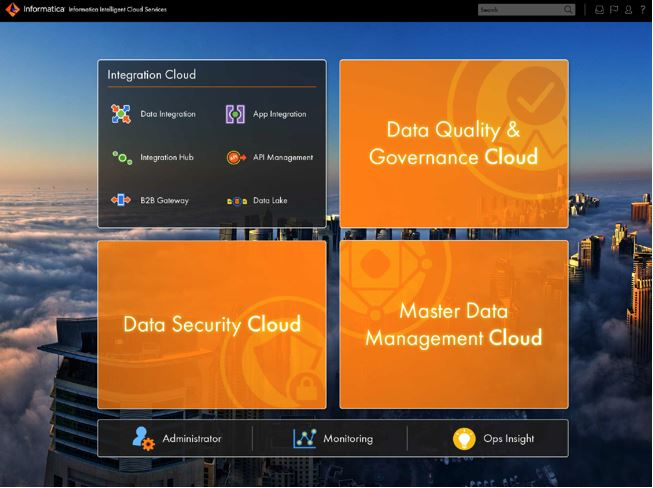
\includegraphics[width=\columnwidth]{images/IICS-0.jpg}
	\caption{IICS Products}\label{f:iics-products}
\end{figure}

\begin{acks}

The author would like to thank Dr.~Gregor~von~Laszewski for his
support and suggestions to write this paper.

\end{acks}

\bibliographystyle{ACM-Reference-Format}
\bibliography{report} 
